\section{Introdução}\label{introduuxe7uxe3o}

Este sensor tem o objetivo de detectar tensão em um fio sem o contato
com o mesmo. Com isso você pode testar se há tensão nos fios de
aparelhos elétricos, em fios de uma tubulação em que você não encontre a
saída ou simplesmente para detectar eletricidade estática de um corpo.

\section{Material Utilizado}\label{material-utilizado}

\begin{itemize}
\itemsep1pt\parskip0pt\parsep0pt
\item
  Protoboard
\item
  Fios
\item
  1 LED Vermelho Standard
\item
  1 Bateria de 9V
\item
  3 Transistores modelo BC546 - B (NPN)
\item
  1 Resistor de 220 $\Omega$
\item
  1 Resistor de 100K $\Omega$
\item
  1 Resistor de 1M $\Omega$
\item
  1 Push Button
\end{itemize}

\subsection{Informações sobre o Transistor
BC546}\label{informauxe7uxf5es-sobre-o-transistor-bc546}

\begin{itemize}
\itemsep1pt\parskip0pt\parsep0pt
\item
  Pacote TO-92
\item
  $V_{CBO} = 80V$
\item
  $V_{CEO} = 65V$
\item
  $V_{EBO} = 6V$
\item
  $I_C = 100mA$ - Corrente do Coletor
\item
  $P_C = 500mW$ - Potência do Coletor
\item
  $T_J = 150 \degree C$ - Temperatura da Junção
\item
  $H_{FE} = 200 \sim 450$ - Classificação B
\end{itemize}

\section{Montagem do Circuito}\label{montagem-do-circuito}

\begin{figure}[H]
    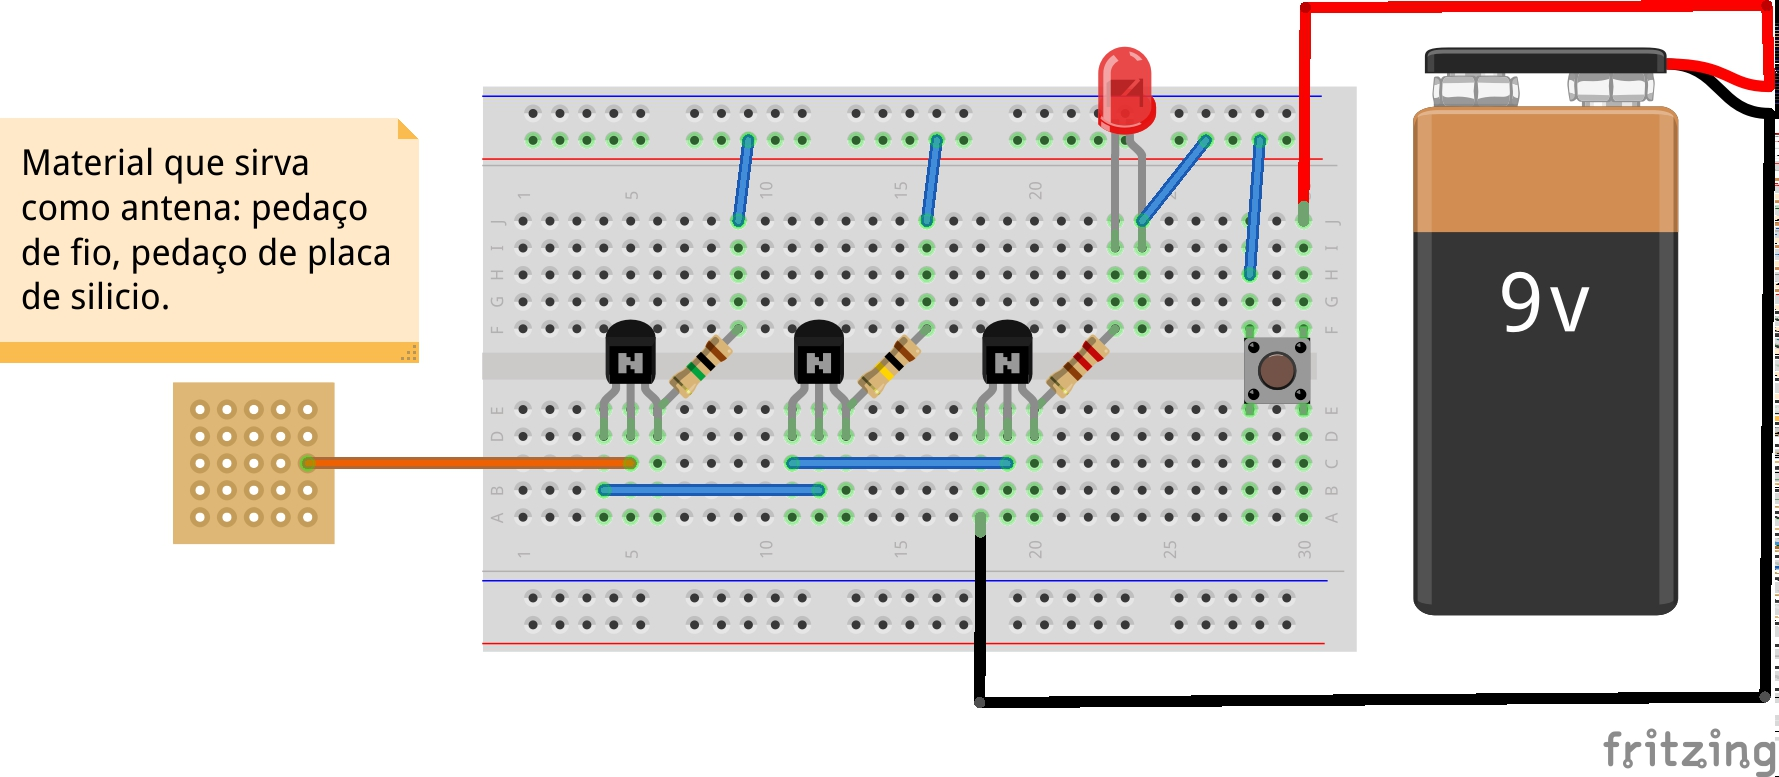
\includegraphics[scale=0.9]{img/non-contact-voltage-sensor_bb.jpg}
    \caption{Montagem Visão Protoboard}
\end{figure}

\subsection{Esquemático}\label{esquemuxe1tico}

\begin{figure}[H]
    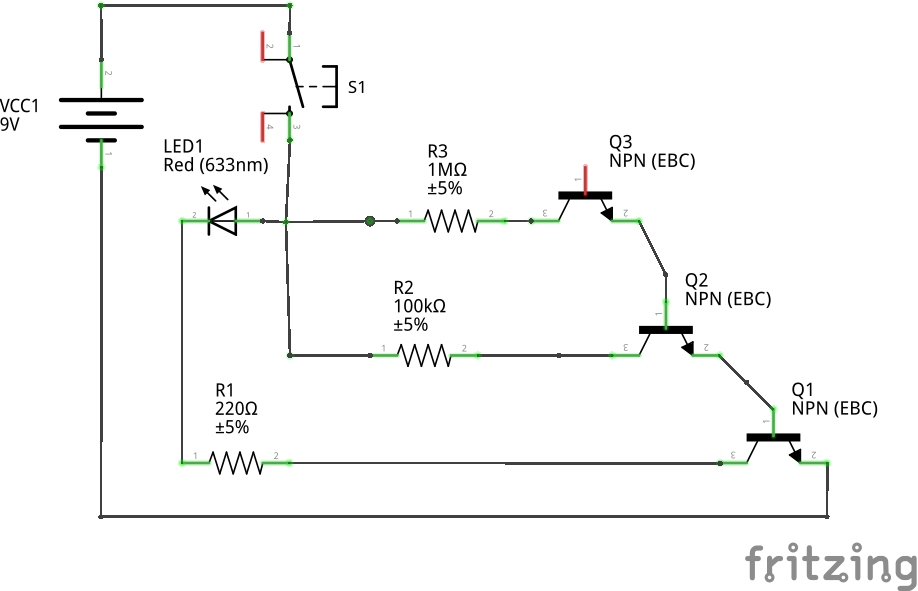
\includegraphics[scale=1.6]{img/non-contact-voltage-sensor_Esquematico.jpg}
    \caption{Esquemático}
\end{figure}

\section{Funcionamento}\label{funcionamento}

\begin{figure}[h]
    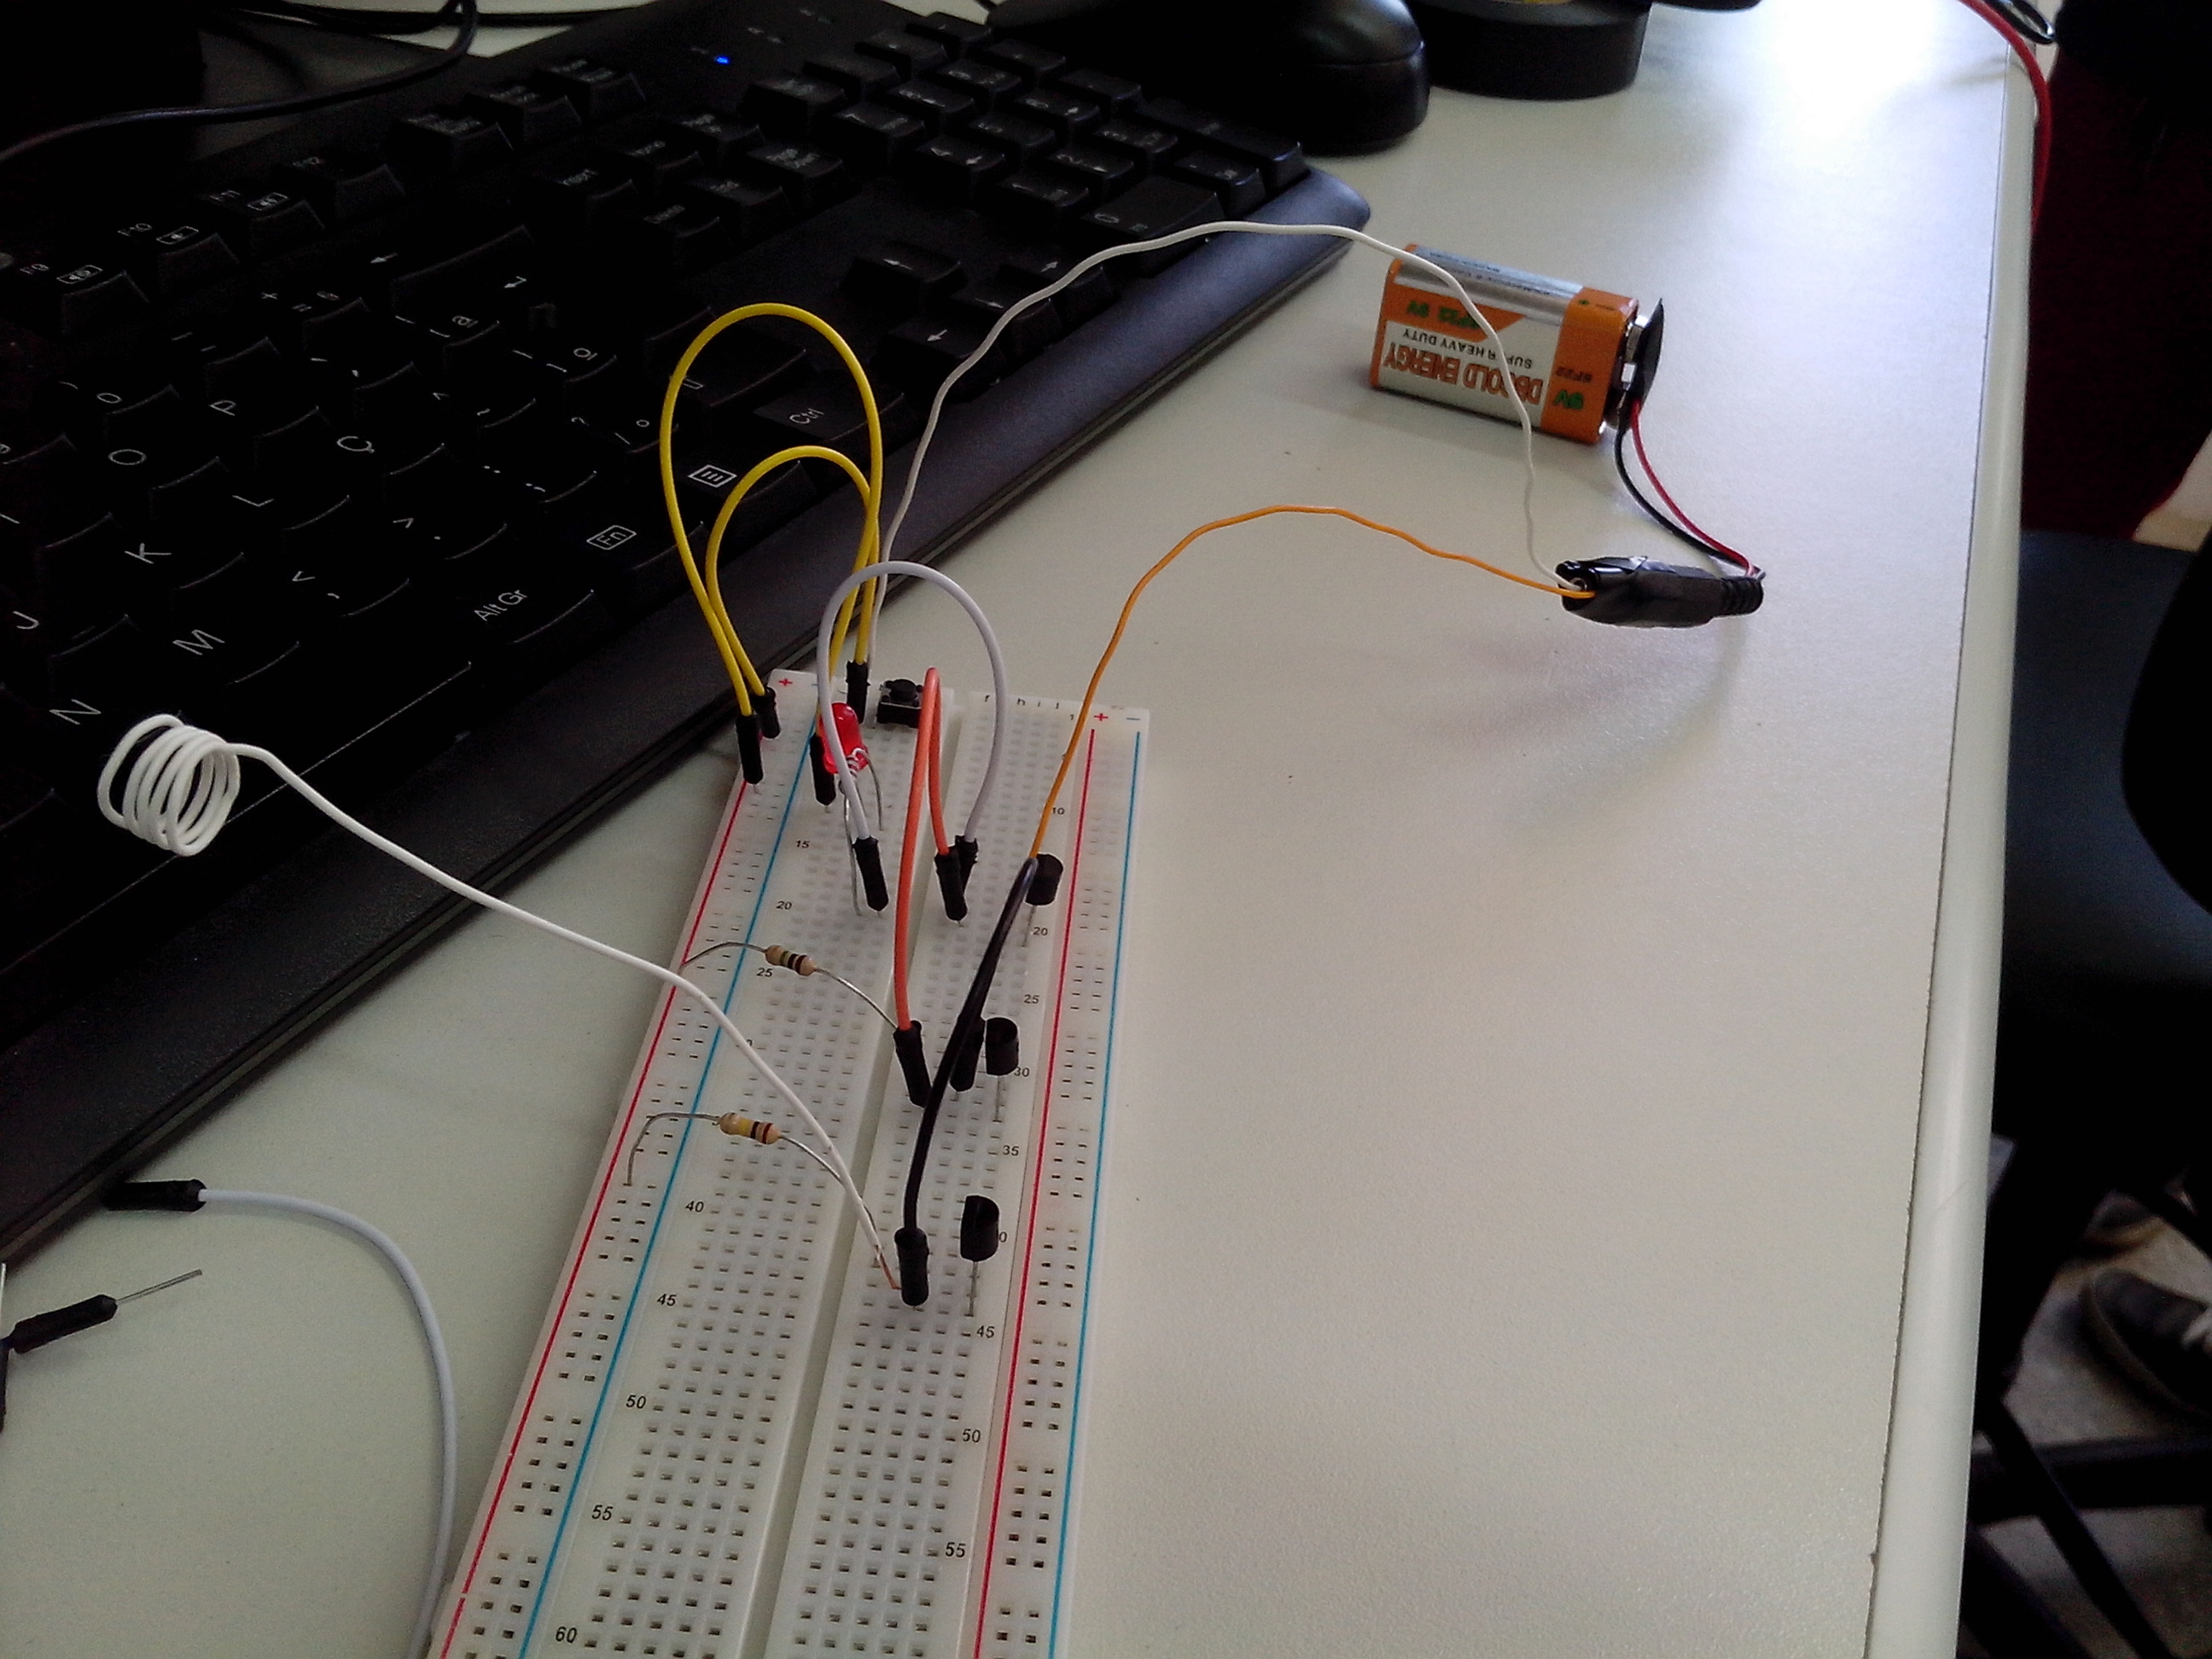
\includegraphics[scale=0.15]{img/IMG_20160521_101811.jpg}
    \caption{Circuito na Protoboard}
\end{figure}

A ideia básica de funcionamento é a seguinte: Ao acionar o \emph{Push
Button} o sistema é energizado e está preparado para detectar tensão.
Para isso é utilizado uma espécie de antena, a qual ao estar próxima a
uma fonte de tensão em que há um campo eletromagnético, potencializa
essa tensão no circuito fazendo com que o LED acenda.

Os Transistores servem como chaves e também tem a função de elevar a
tensão. Se você usar a saída de um transistor para controlar outro, o
ganho multiplica. Com dois transistores, o ganho ideal ($H_{FE} = 200$)
torna-se $200 \times 200 = 40000$, com 3 transistores, o ganho chega a
$200 \times 200 \times 200 = 8000000$! É um ganho altíssimo e permite
que o circuito seja usado para detectar o menor dos movimentos de
eletricidade - mesmo aqueles criados à distância por indução ou
eletricidade estática!

\section{Conclusão}\label{conclusuxe3o}

Com um circuito simples com zero de programação por software é possível
criar um detector de tensão usando somente a física. Com esse exemplo
prático é possível comprovar a existência de campos eletromagnéticos.

\textbf{Observação}: Apesar de tudo não use este circuito em
equipamentos de alta tensão, mesmo que ele indique que não há tensão.
Você pode correr riscos ao manipular estes equipamentos. Na dúvida evite
o contato.

Também não utilize perto de fios desencapados, ou diretamente no plug da
tomada. Também a riscos de choque nesses casos.

\section{Bibliografia}\label{bibliografia}

\begin{itemize}
\itemsep1pt\parskip0pt\parsep0pt
\item
  Non-Contact Voltage Detector
\end{itemize}

\url{http://makezine.com/projects/non-contact-voltage-detector/}

\begin{itemize}
\itemsep1pt\parskip0pt\parsep0pt
\item
  BC546/547/548/549/550 Fairchild Datasheet
\end{itemize}

\url{http://www.electroschematics.com/wp-content/uploads/2012/06/BC546-BC547-BC548-BC549-BC550-datasheet.pdf}
